\subsection{Zugrundeliegende Physik}
Laser (kurz für \textit{light amplification by stimulated emission of radiation}) machen sich die Wechselwirkung zwischen Photonen und Hüllenelektronen zunutze. Dabei gibt es drei grundlegende Phänomene (erklärt am Beispiel eines Zweiniveausystems mit Energiedifferenz $E$):
\begin{itemize}
	\item Absorption: Das Elektron ist auf dem unteren Niveau. Ein einfallendes Photon mit Energie $E$ gibt seine gesamte Energie an das Elektron ab, das somit auf das obere Niveau gelangt. Das Atom ist nun angeregt.
	\item Induzierte Emission: Das Elektron ist auf dem oberen Niveau. Ein einfallendes Photon, das etwa die Energie $E$ hat, verursacht die Emission eines zweiten Photons mit Energie $E$ beim Übergang des Elektrons zum unteren Niveau.
	\item Spontane Emission: Das Elektron ist auf dem oberen Niveau und emittiert spontan, zur Energieminimierung, ein Photon der Energie $E$.
\end{itemize}
Die Besetzungsdichten der beiden Niveaus $n_1,n_2$ können mit folgenden Differentialgleichungen beschrieben werden
\begin{align}\label{eq:DGL}
	\dot{n}_1 &= - n_1B_{12}\rho(x) + n_2B_{21}\rho(x) + n_2A_{21} \nonumber\\
	\dot{n}_2 &= + n_1B_{12}\rho(x) - n_2B_{21}\rho(x) - n_2A_{21}
\end{align}
$\rho(x)$ ist dabei die Energiedichte des einfallenden Strahlungsfelds und $A_{21}, B_{12}, B_{21}$ die Einsteinkoeffizienten und dienen als Maß für die Wahrscheinlichkeit eines Übergangs. \\
Man spricht von Besetzungsinversion, wenn die Besetzung des oberen Niveaus $n_2$ größer ist, als die des unteren $n_1$, mit anderen Worten, wenn die Differenz der beiden Besetzungsdichten $\Delta N = n_1-n_2$ negativ ist. Durch Transformation der Variablen $n_1,n_2$ zu $\Delta N, N=n_1+n_2=const$ in den Gleichungen \eqref{eq:DGL} und Lösung der neuen Differentialgleichung ergibt sich der Ausdruck
\begin{align}
	\Delta N(t) = N \left[ -\left(\frac{1}{2\frac{B\rho}{A_{21}}+1}+1\right)
	 e^{-\left(B\rho+\frac{A_{21}}{2}\right)t} + \frac{1}{2\frac{B\rho}{A_{21}}+1} \right]\ ,
\end{align}
wenn $\Delta N(0) = -N$, d.h. alle Atome angeregt sind, und die Niveaus nicht entartet, d.h. $B_{12}=B_{21}=B$, sind. Für lange Zeiten konvergiert $\Delta N$ gegen $N\slash(2\frac{B\rho}{A_{21}}+1) > 0$, d.h. eine dauerhafte Besetzungsinversion kann mit einem Zweiniveausystem nicht erreicht werden.
\subsection{Grundsätzlicher Aufbau und Funktionsweise}
Bestimmend für die Frequenz des Laserlichts ist das Lasermedium. Durch eine äußere Energiequelle wird die Emission von Photonen im Medium angeregt und aufrecht erhalten, hierbei ist auch von \textit{pumpen} die Rede. Um einen kohärenten und starken Laserstrahl zu erhalten ist es dann wichtig, dass das Strahlungsfeld ständig verstärkt wird. Um das zu erreichen ist eine dauerhafte Besetzungsinversion nötig. Dafür wird ein Resonator verwendet. Er besteht aus zwei sich gegenüber stehenden Spiegeln, wovon einer teilreflektierend sein sollte um den Laserstrahl auskoppeln zu können, mit dem Lasermedium in der Mitte. Er sorgt dafür, dass die emittierten Photonen das Medium mehrfach durchlaufen und so Atome anregen können oder durch stimulierte Emission das Strahlungsfeld verstärken. Die grundsätzliche Anordnung der Bauteile ist in Abbildung \ref{fig:BasicLaser} dargestellt.
\begin{figure}[h!]
	\centering
	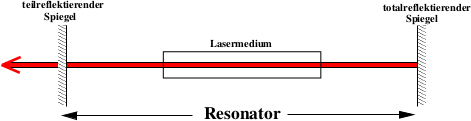
\includegraphics[width=.6\textwidth]{BasicAufbau.png}
	\caption{Schematischer Aufbau eines Lasers \cite{V61}}
	\label{fig:BasicLaser}
\end{figure} \\
Die Form der Resonatorspiegel kann verschieden sein und entscheidet über die Stabilität des Lasers. Als Kenngröße dient dabei $g_i = 1-\frac{L}{r_i}$, die einen Zusammenhang zwischen dem Krümmungsradius des Spiegels $r_i$ der Länge $L$ des Resonators herstellt. Eingesetzt in die resonator-spezifische Funktion $g(L) = g_1 \cdot g_2$ erhält man beispielsweise 
\begin{align}
	&g(L) = \frac{1}{r_1r_2}L^2 - \left(\frac{1}{r_1}+\frac{1}{r_2}\right)L + 1 &&\text{\small wenn beide Spiegel gekrümmt,} \\
	&g(L) = 1-\frac{L}{r_2} &&\text{\small wenn ein Spiegel planar, der andere gekrümmt ist.}
\end{align}
Ein Resonator ist optisch stabil, wenn 
\begin{align}\label{eq:Stabilitat}
	0\leq g(L) <1
\end{align}
gilt.
Auch die Moden der stehenden Welle, die sich im Resonator ausbildet, haben einen Einfluss auf die Verluste. Sie werden als $\text{TEM}_{lp}$-Moden bezeichnet, wobei $l,p$ die Anzahlen der Knoten in $x,y$- -- also transversaler -- Richtung sind. Die sogenannte $\text{TEM}_{00}$-Mode ist hierbei die präferierte, denn sie hat keine transversalen Anteile, welche die Fokussierung erschweren. Ihre Intensitätsverteilung auf einem Schirm wird durch die Gaußverteilung
\begin{align}
	I(r) = I_0\exp\left(-2\left(\frac{r}{\omega}\right)^2\right)
\end{align}
mit dem Abstand zur optischen Achse $r$ und dem Strahldurchmesser $2\omega$ beschrieben. Der Strahlradius $\omega$ hängt von der Fokussierung ab und kann mit
\begin{align}
	\omega(z) = \omega_0\sqrt{1+\left(\frac{\theta z}{\omega_0}\right)^2}
\end{align}
moduliert werden, wobei $\theta = \omega_0\lambda\slash\pi$ die Divergenz des Strahls ist. \\
\ \\
Neben den beschriebenen grundlegenden Bauteilen werden weitere Elemente zur Verbesserung des Strahls eingesetzt:
\begin{itemize}
	\item Brewsterfenster an beiden Seiten der Kammer, die das Lasermedium enthält, sorgen für die Polarisation des Lichts. Sie bestehen aus Glasplatten, die im Brewsterwinkel zum Strahl stehen und so die senkrecht polarisierten Anteile der Welle herausfiltern.
	\item Modenblenden sind mechanische Widerstände, die transversale Moden blockieren. WO WERDEN DIE HINGESTELLT?
\end{itemize}
\subsection{Der HeNe-Laser}
Beim HeNe-Laser befindet sich neben Neon als Lasermedium noch Helium als Pumpgas im Verhältnis 1 (Ne) zu 5 (He). Die Heliumatome werden durch Entladung angeregt. Durch Stöße zweiter Art ($A^* + B \rightarrow A + B^*$) werden die Neonatome angeregt. Das Energieniveauschema \ref{fig:Niveaus} stellt diesen und die darauf folgenden Abläufe in den Atomhüllen dar. Die intensivste der emittierten Wellenlängen, ist rote mit einer Wellenlänge von $\lambda = \SI{632.8}{\nano\metre}$.
\begin{figure}[h!]
	\centering
	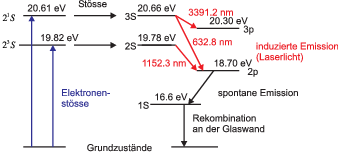
\includegraphics[width=.6\textwidth]{Niveauschema.png}
	\caption{Niveauschema der Abläufe im HeNe-Laser \cite{Niveaus}}
	\label{fig:Niveaus}
\end{figure}